

% ------------------------------------------------------------------------------
% ------------------------------------------------------------------------------

%
% Optional reading
%

\begin{frame}[plain,c]
\begin{center}
{\Huge \bf Optional reading for Lecture \thislecture}
\end{center}
\end{frame}


%
%
%

\begin{frame}{Electric dipole field}

\begin{columns}
  \begin{column}{0.20\textwidth}
   \begin{center}
     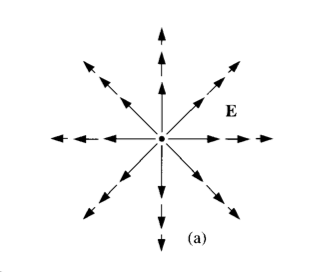
\includegraphics[width=0.99\textwidth]{./images/schematics/electric_field_pos_point_charge.png}\\
   \end{center}
  \end{column}
  \begin{column}{0.80\textwidth}
     As we know, the potential field $V(\vec{r})$ due to an
     {\bf electric monopole} (i.e. a point charge q) has an $1/r$ dependence:
     \begin{equation*}
         V = \frac{1}{4\pi\epsilon_0} \frac{q}{r}
     \end{equation*}
     Consequently, its electric field $\vec{E}(\vec{r})$ ($\vec{E} = -\vec{\nabla}V$)
     has an $1/r^2$ dependence.
  \end{column}
\end{columns}

\vspace{0.3cm}

\begin{columns}
  \begin{column}{0.80\textwidth}
     We will see that the potential field $V(\vec{r})$ due to an {\bf electric dipole} is
     \begin{equation*}
        {\bf V \approx \frac{1}{4\pi\epsilon_0} \frac{\vec{p} \hat{r}}{r^2} }
     \end{equation*}
     Therefore, it falls off as $1/r^2$, faster than the monopole potential.
     Consequently, the dipole electric field $\vec{E}(\vec{r})$
     has an $1/r^3$ dependence.
  \end{column}
  \begin{column}{0.20\textwidth}
   \begin{center}
     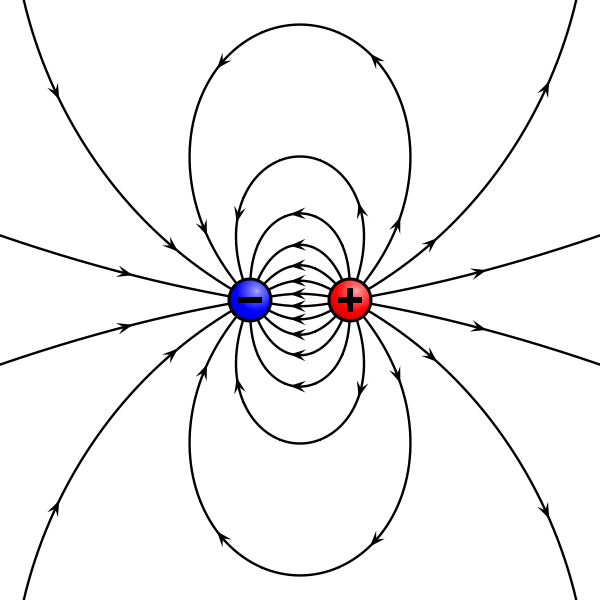
\includegraphics[width=0.90\textwidth]{./images/schematics/electric_dipole_field_lines_2.png}\\
   \end{center}
  \end{column}
\end{columns}

\end{frame}


%
%
%

\begin{frame}{Calculating the electric dipole field}

As we know, the potential field due to a single charge q is given by:
\begin{equation*}
  V = \frac{1}{4\pi\epsilon_0} \frac{q}{r}
\end{equation*}

\vspace{0.1cm}

\begin{columns}
  \begin{column}{0.25\textwidth}
   \begin{center}
     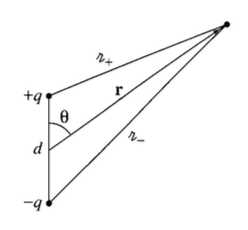
\includegraphics[width=0.95\textwidth]{./images/schematics/electric_dipole_0.png}\\
   \end{center}
  \end{column}
  \begin{column}{0.75\textwidth}
    Now, I have 2 charges: a positive and a negative one. The superposition principle applies.
    The potential at a distance r from the centre of the dipole is:
    \begin{equation*}
      V = \frac{1}{4\pi\epsilon_0} \Big( \frac{q}{r_{+}} - \frac{q}{r_{-}} \Big)
    \end{equation*}
  \end{column}
\end{columns}

\vspace{0.1cm}

I need to express $r_{+}$ and $r_{-}$ in terms of r.
From the law of cosines (generalisation of the Pythagorean theorem):
\begin{equation*}
  r_{+}^{2} = r^{2} + (d/2)^{2} - r \cdot d \cdot cos\theta
            = r^{2} \Big( 1 - \frac{d}{r} cos\theta + \frac{d^2}{4r^2} \Big) \xRightarrow{r>>d}
\end{equation*}
\begin{equation*}
   r_{+}^{2} \approx r^{2} \Big( 1 - \frac{d}{r} cos\theta \Big)
\end{equation*}

\end{frame}

%
%
%

\begin{frame}{Calculating the electric dipole field}

For $r_{-}$, the expressions are similar but involves $cos(\pi - \theta) = -cos\theta$ and,
therefore, there is an extra minus sign.
\begin{equation*}
   r_{-}^{2} \approx r^{2} \Big( 1 + \frac{d}{r} cos\theta \Big)
\end{equation*}

For convenience let me rename the small term involving d/r as $\epsilon$:
\begin{equation*}
  \frac{d}{r} cos\theta = \epsilon
\end{equation*}

We have that
\begin{equation*}
   r_{+}^{2} \approx r^{2} (1 - \epsilon) \Rightarrow
   r_{+} \approx r (1 - \epsilon)^{1/2} \Rightarrow
   \frac{1}{r_{+}} \approx \frac{1}{r} (1 - \epsilon)^{-1/2} \Rightarrow
   \frac{1}{r_{+}} \approx \frac{1}{r} (1 + \frac{1}{2}\epsilon)
\end{equation*}

and, similarly
\begin{equation*}
   \frac{1}{r_{-}} \approx \frac{1}{r} (1 - \frac{1}{2}\epsilon)
\end{equation*}

\end{frame}

%
%
%

\begin{frame}{Calculating the electric dipole field}

Therefore
\begin{equation*}
  \frac{1}{r_{+}} - \frac{1}{r_{-}} \approx
    \Big( \frac{1}{r} (1 + \frac{1}{2}\epsilon) \Big) -
    \Big( \frac{1}{r} (1 - \frac{1}{2}\epsilon) \Big) =
    \frac{1}{r} \epsilon \xRightarrow{\epsilon = \frac{d}{r} cos\theta}
\end{equation*}
\begin{equation*}
  \frac{1}{r_{+}} - \frac{1}{r_{-}} \approx \frac{d}{r^2} cos\theta
\end{equation*}

The electric dipole potential is given by
\begin{equation*}
  V = \frac{1}{4\pi\epsilon_0} \Big( \frac{q}{r_{+}} - \frac{q}{r_{-}} \Big) \Rightarrow
  V \approx \frac{1}{4\pi\epsilon_0} \frac{q d cos\theta}{r^2} \Rightarrow
\end{equation*}
\begin{equation*}
  V \approx \frac{1}{4\pi\epsilon_0} \frac{\vec{p} \cdot \hat{r}}{r^2}
\end{equation*}

So the potential of a dipole falls off as $1/r^2$ ($1/r$ for a monopole).\\
Consequently, the electric field of a dipole falls off as $1/r^3$.\\

\end{frame}

% ------------------------------------------------------------------------------

%
%
%

\begin{frame}{The {\em multipole} expansion}

\begin{columns}
  \begin{column}{0.30\textwidth}
   \begin{center}
     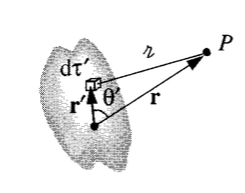
\includegraphics[width=0.99\textwidth]{./images/schematics/continuous_charge_distribution_1.png}\\
   \end{center}
  \end{column}
  \begin{column}{0.70\textwidth}
    For an {\bf arbitrary charge distribution} characterised by a density $\rho$
    the potential can be expanded to:
    \begin{equation*}
      V(r) = \frac{1}{4\pi\epsilon_0} \sum_{n=0}^{\infty} \frac{1}{r^{n+1}}
        \int_{vol} (r^{\prime})^{n} P_{n}(cos\theta^{\prime}) \rho(\vec{r^{\prime}}) d{\tau}^{\prime}
    \end{equation*}
    where $\theta^{\prime}$ is the angle between $\vec{r}$ and $\vec{r^{\prime}}$.
    Notice that there is no r dependence in the integral.\\
  \end{column}
\end{columns}

\vspace{0.3cm}

This is called the {\bf multipole expansion}.
\begin{itemize}
{\small
  \item The first ($1/r$) term is the {\bf monopole} term
  \item The second ($1/r^2$) term is the {\bf dipole} term
  \item $1/r^3$ term: {\bf quadruple} term
  \item $1/r^4$ term: {\bf octopole} term
  \item ...
}
\end{itemize}

\end{frame}

% ------------------------------------------------------------------------------

%
% Worked example : The not-so-parallel plate capacitor
%

{
\problemslide

\begin{frame}{Worked example: The not-so-parallel plate capacitor}

  \begin{blockexmplque}{Question}
  In the figure below, you are given the not-so-parallel plate capacitor.
  \begin{itemize}
    \item
     Neglecting edge effects, when a voltage difference $V_0$ is placed
     across the two conductors, find the potetial everywhere between the plates.
    \item
     When the wedge is filled with a medium of dielectric constant $\epsilon$,
     find the capacitance of the system in terms of the constants given.
  \end{itemize}
  \begin{center}
    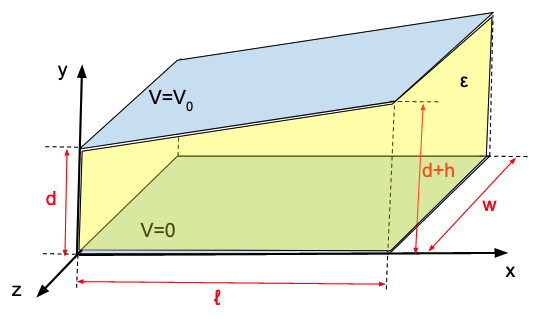
\includegraphics[width=0.60\textwidth]{./images/problems/lect4_not_so_parallel_plane_capacitor_1.png}\\
  \end{center}
  \end{blockexmplque}

\end{frame}

%
%
%

\begin{frame}{Worked example: The not-so-parallel plate capacitor}

Neglecting edge effects, the problem is a two-dimensional one.\\
\vspace{0.1cm}
Symmetry dictates that the electric field is parallel to the $xy$ plane
and it is {\em independent} of $z$.\\
\vspace{0.1cm}
A convenient coordinate system for our analysis is $O^\prime (x^\prime, y^\prime, z^\prime)$
which is shifted from $O (x, y, z)$ by a distance $\ell^\prime$ along the $x$ axis,
so imaginary extrapolations of the capacitor plates
intersect at $x^\prime=0$, as shown below.

\begin{center}
  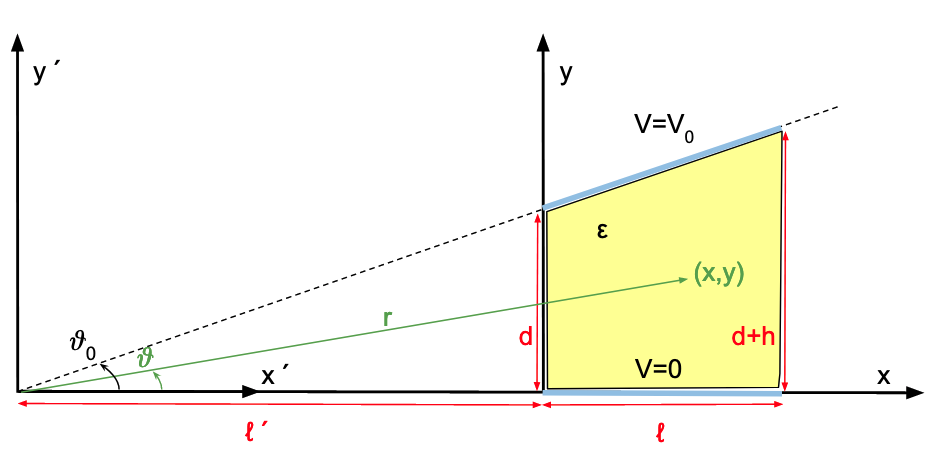
\includegraphics[width=0.80\textwidth]{./images/problems/lect4_not_so_parallel_plane_capacitor_2.png}\\
\end{center}

\end{frame}


%
%
%

\begin{frame}{Worked example: The not-so-parallel plate capacitor}

The quantities $\ell^\prime$, $\theta_0$, $\theta$ and $r$ introduced above (see schematic)
can be easily related to the given quantities $\ell$, $d$, $h$ and the coordinates $x,y$
of a point within the capacitor in the original coordinate system ($O$).

  \begin{equation*}
    tan\theta_0 = \frac{d+h}{\ell+\ell^\prime} = \frac{d}{\ell^\prime} \Rightarrow
     \ell^\prime = \ell \frac{d}{h}
  \end{equation*}

  \begin{equation*}
    tan\theta_0 = \frac{d}{\ell^\prime} = \frac{\cancel{d}}{\ell \frac{\cancel{d}}{h}} \Rightarrow
    \theta_0 = arctan\Big(\frac{h}{\ell}\Big)
  \end{equation*}

  \begin{equation*}
    tan\theta = \frac{y}{x+\ell^\prime} = \frac{y}{x+\ell \frac{d}{h}} \Rightarrow
    \theta = arctan\Big(\frac{y}{x+\ell \frac{d}{h}}\Big)
  \end{equation*}

  \begin{equation*}
    cos\theta = \frac{x+\ell^\prime}{r} = \frac{x+\ell \frac{d}{h}}{r} \xRightarrow{\; cos\theta \approx 1 \;}
    r = x + \ell \frac{d}{h}
  \end{equation*}

\end{frame}

%
%
%

\begin{frame}{Worked example: The not-so-parallel plate capacitor}

The potetial between the plates can be found by solving Poisson's equation

  \begin{equation*}
    \vec{\nabla}^{2} V = \frac{\rho}{\epsilon_0} \xRightarrow{\rho=0}
    \vec{\nabla}^{2} V = 0
  \end{equation*}

In polar coordinates, this is written as

  \begin{equation*}
    \frac{1}{r^2} \frac{d^2V(\theta)}{d\theta} = 0 \Rightarrow
    \frac{d^2V(\theta)}{d\theta} = 0
  \end{equation*}

\vspace{0.2cm}

The equation has the following solution

  \begin{equation*}
    V(\theta) = A + B \theta
  \end{equation*}

The costants $A, B$ can be derived from the boundary conditions

  \begin{equation*}
    V(\theta = 0) = 0 \Rightarrow A = 0
  \end{equation*}

  \begin{equation*}
    V(\theta = \theta_0) = V_0 \xRightarrow{A = 0}
    B \theta_0 = V_0 \Rightarrow B = \frac{V_0}{\theta_0}
  \end{equation*}

\end{frame}

%
%
%

\begin{frame}{Worked example: The not-so-parallel plate capacitor}

Therefore, the solution $V(\theta)$ is given by

  \begin{equation*}
    V(\theta) =  \frac{V_0}{\theta_0} \theta
  \end{equation*}

Using the expression for $\theta_0$ that was derived previously,
$V(\theta)$ can be written as

  \begin{equation*}
    V(\theta) =  \frac{V_0}{arctan\Big(\frac{h}{\ell}\Big)} \theta
  \end{equation*}

In terms of coordinates $x,y$ in the original coordinate system ($O$),
the potential can be expressed as

  \begin{equation*}
    V(x,y) =  \frac{V_0}{arctan\Big(\frac{h}{\ell}\Big)}
     \arctan\Big(\frac{y}{x+\ell \frac{d}{h}}\Big)
  \end{equation*}

\end{frame}

%
%
%

\begin{frame}{Worked example: The not-so-parallel plate capacitor}

The capacitance of the system will be calculated from
  \begin{equation*}
    C = \frac{|Q|}{|V_0|}
  \end{equation*}

where the unknown charge $Q$ can be estimated from
  \begin{equation*}
    Q = \oint \vec{D} \cdot d\vec{S}
  \end{equation*}

The field $\vec{D}$ is related to electric field $\vec{E}$,
and therefore the potential V, as
  \begin{equation*}
    \vec{D} = \epsilon \vec{E} \xRightarrow{\vec{E} = -\vec{\nabla}V}
    \vec{D} = -\epsilon \vec{\nabla}V
  \end{equation*}

Therefore
  \begin{equation*}
    \vec{D} =
      -\epsilon \frac{1}{r} \frac{\partial V}{\partial \theta} \hat{\theta}
      \xRightarrow{\;V =  \frac{V_0}{\theta_0} \theta \;}
    \vec{D} = - \frac{1}{r} \frac{\epsilon V_0}{\theta_0} \hat{\theta}
  \end{equation*}

\end{frame}

%
%
%

\begin{frame}{Worked example: The not-so-parallel plate capacitor}

Using the above expression for $\vec{D}$, $Q$ is calculated as
  \begin{equation*}
    Q = \oint \vec{D} \cdot d\vec{S} = \oint D dS
     \xRightarrow{\; dS = w dx, \; D = - \frac{1}{r} \frac{\epsilon V_0}{\theta_0} \;}
     Q = -\frac{w \epsilon V_0}{\theta_0} \int_{0}^{\ell} \frac{1}{r} dx
      \xRightarrow{\; r = x + \ell \frac{d}{h} \;}
  \end{equation*}

  \begin{equation*}
    Q = -\frac{w \epsilon V_0}{\theta_0} \int_{0}^{\ell} \frac{1}{x + \ell \frac{d}{h}} dx =
        -\frac{w \epsilon V_0}{\theta_0} ln(x + \ell \frac{d}{h}) \Big\rvert_{0}^{\ell} \Rightarrow
  \end{equation*}

  \begin{equation*}
    Q = -\frac{w \epsilon V_0}{\theta_0} ln \frac{d + h}{d}
    \xRightarrow{\theta_0 = arctan\Big(\frac{h}{\ell}\Big)}
    Q = -\frac{w \epsilon V_0}{arctan\Big(\frac{h}{\ell}\Big)} ln \Big(\frac{d + h}{d}\Big)
  \end{equation*}

Therefore
  \begin{equation*}
    C = \frac{|Q|}{|V_0|} =
      \frac{w \epsilon}{arctan\Big(\frac{h}{\ell}\Big)} ln \Big(\frac{d + h}{d}\Big)
  \end{equation*}

\end{frame}


} % Worked example

% ------------------------------------------------------------------------------

%
% Worked example : Pulling a dielectric out of a capacitor
%

{
\problemslide

\begin{frame}{Worked example: Pulling a dielectric out of a capacitor}

  \begin{blockexmplque}{Question}
  A cylindrical capacitor of length $L$ consists of an inner metallic wire
  of radius $a$, and a thin outer metallic shell of radius $b$.
  The space in between is filled with a dielectric with permittivity $\epsilon$.\\
  As we have seen in the workshops, if edge effects are ignored,
  the capacitance $C$ of the cylindrical
  capacitor is given by
  \begin{equation*}
    C = \frac{2\pi \epsilon L}{ln(b/a)}.
  \end{equation*}
  \vspace{0.2cm}
  Suppose that the dielectric is pulled partly out of the capacitor,
  and that the capacitor is connected to a battery of electromotive force $V$.
  \begin{enumerate}
  \item
  Find the force necessary to hold the dielectric in this position.
  \item
  In which direction must the force be applied?\\
  \end{enumerate}
  \end{blockexmplque}

\end{frame}

%
%
%

\begin{frame}{Worked example: Pulling a dielectric out of a capacitor}

  \begin{center}
    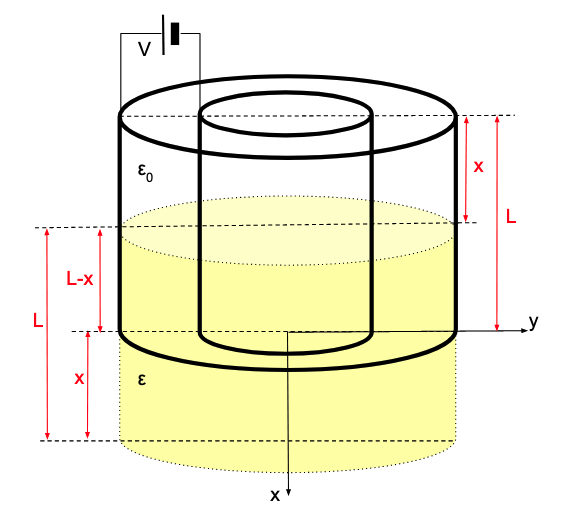
\includegraphics[width=0.67\textwidth]{./images/problems/lect4_pulling_dielectric_out_of_capacitor_1.png}\\
  \end{center}

\end{frame}

%
%
%

\begin{frame}{Worked example: Pulling a dielectric out of a capacitor}

  If the dielectric is pulled out of the cylindrical capacitor by a length $x$,
  then length $L-x$ remains inside the capacitor.

  The part of the capacitor with length $x$ that does not have a dielectric
  has capacitance $C_1$ given by
  \begin{equation*}
    C_1 = \frac{2\pi \epsilon_0 x}{ln(b/a)}
  \end{equation*}
  whereas the part of the capacitor with length $L-x$ that does have a
  dielectric has a capacitance $C_2$ given by
  \begin{equation*}
    C_2 = \frac{2\pi \epsilon (L-x)}{ln(b/a)}.
  \end{equation*}

  Those two capacitors have a common potential difference across the
  inner and outer conductors (connected parallel) and, therefore, the
  combined capacitance $C$ is
  \begin{equation*}
    C = C_1 + C2 =
     \frac{2\pi \epsilon_0 x}{ln(b/a)} +
     \frac{2\pi \epsilon (L-x)}{ln(b/a)} =
     \frac{2\pi \epsilon}{ln(b/a)}
         \Big(L + (\frac{\epsilon_0}{\epsilon}-1) x \Big)
  \end{equation*}

\end{frame}

%
%
%

\begin{frame}{Worked example: Pulling a dielectric out of a capacitor}

  The work provided by the battery as it charges the capacitor
  becomes energy stored in the capacitor and mechanical work of
  the force $F$ that moves the dielectric with respect to the capacitor.
  We can write
  \begin{equation*}
    dW_{battery} = dU_{capacitor} + dW_{mechanical} \Rightarrow
  \end{equation*}
  \begin{equation*}
    V dQ = d\Big(\frac{1}{2}CV^2\Big) + F dx
  \end{equation*}
  Since $V$ is constant, the above can be written as
  \begin{equation*}
    V dQ = \frac{1}{2}V^2 dC + F dx
  \end{equation*}
  Using the definition of capacitance, $C = \frac{Q}{V}$, we can write
  \begin{equation*}
    dC = \frac{dQ}{V} \Rightarrow V^2 dC = V dQ
  \end{equation*}
  From all the above, we obtain
  \begin{equation*}
    V^2 dC = \frac{1}{2}V^2 dC + F dx \Rightarrow
    \frac{1}{2}V^2 dC = F dx
  \end{equation*}

\end{frame}

%
%
%

\begin{frame}{Worked example: Pulling a dielectric out of a capacitor}

  As the dielectric exits the capacitor, $x$ increases
  and, therefore, $dx > 0$.

  When $x$ increases we expect the capacitance $C$ to decrease.
  Given that $\epsilon_0/\epsilon < 1$,
  this can be easily deduced from the expression for $C$,
  \begin{equation*}
    C =
     \frac{2\pi \epsilon}{ln(b/a)}
         \Big(L + (\frac{\epsilon_0}{\epsilon}-1) x \Big).
  \end{equation*}
  Therefore, for $dx > 0$, $dC < 0$.
  Considering this and observing the expression
  \begin{equation*}
    \frac{1}{2}V^2 dC = F dx,
  \end{equation*}
  we see that the term $F dx$ needs to be negative.
  Therefore, for $dx > 0$ (direction of exiting the capacitor),
  the direction of the force on the dielectric is opposite,
  and the dielectric is pulled into the capacitor.

  If we wanted to hold the dielectric in a fixed position, we would
  need to apply an opposite force $\vec{F^\prime}(=-\vec{F})$,
  pointing {\em away} from the capacitor.

\end{frame}

%
%
%

\begin{frame}{Worked example: }

  The magnitude of my force $F^\prime=F$
  \begin{equation*}
    \frac{1}{2}V^2 dC = F dx \Rightarrow
    F = \frac{1}{2}V^2 \frac{dC}{dx}
  \end{equation*}

  Differentiating the expression for $C$ we derived earlier, we find
  \begin{equation*}
    \frac{dC}{dx} = \frac{2\pi \epsilon}{ln(b/a)}
        \Big(\frac{\epsilon_0}{\epsilon}-1\Big)
  \end{equation*}

  Thefore, the magnitude of the force is given by
  \begin{equation*}
    F = \frac{1}{2}V^2 \frac{2\pi \epsilon}{ln(b/a)}
     \Big(\frac{\epsilon_0}{\epsilon}-1\Big) \Rightarrow
    F = \frac{\pi \epsilon V^2}{ln(b/a)}
      \Big(\frac{\epsilon_0}{\epsilon}-1\Big)
  \end{equation*}

\end{frame}

} % Worked example
